\documentclass{subfiles}

\begin{document}
    \marginnote{\textit{\textbf{VL 17}}\\26.06.2023\\11:45}

    Um die Wechselwirkung des Spins mit dem Magnetfeld zu beschreiben, wechseln wir in die semiklassische Betrachtungsperspektive. Gehe hierzu über in das Bezugssystem des sich um den Kern bewegenden Elektrons. Für eine mit Strom $I$ durchflossene Kurve, hier die Flugbahn des Elektrons, mit eingeschlossener Fläche $A$ ergibt sich nach Biot Savart das Magnetfeld
    \[
        B(v) = \fdef{
            \frac{\mu_0\cdot Ze}{4\pi\cdot \dabs{r}{2}^3}\cdot(v \times r)
        }{r\in\R^3}\in L_S(\R^3)
    \]
    mit $v\in\R^3$ als Rotationsgeschwindigkeit.  
    \begin{Aufgabe}
        \nr{} Die hier angedeutete Transformation der Koordinatensysteme ist nach relativistischer Einsicht nicht mehr einfach. Führe die Berechnung unter Berücksichtigung der Lorentz Transformation durch. Verifiziere den Zusammenhang der beiden Lösungen durch den Faktor $1/2$ (\href{https://en.wikipedia.org/wiki/Thomas_precession}{\emph{Thomas Faktor}}). 

        \nr{} Zeige nun, daß es sich bei $B:\R^3\to(\Abb{\R^3}{\R^3})$ tatsächlich um eine Abbildung in den Operatorraum der linearen stetigen Operatoren $L_S(\R^3)\subset\Abb{\R^3}{\R^3}$ handelt.

        \nr{EnKorr} Bestimme den Energiekorrekturterm $E_{J,S}$ für das Magnetfeld. Im Ergebnis sollte er sich auf $E_{J,S} = 2\mu_B/\hbar\cdot \sum_{i\in[3]}S_i\circ (B_J)_i$ belaufen, wobei 
    \end{Aufgabe}
    
    \noindent Transformieren wir $B(v)$ nun zu $B(J)$ mit $J = m_e\cdot (r\times v)$ als Drehimpulsoperator in $L_S(\R^3)$ und $m_e\in\R$ als Masse des Elektrons, so erhalten wir den Zusammenhang 
    \[
        B(J) = \fdef{
            \frac{\mu\cdot Z\cdot e}{4\pi\cdot \dabs{r}{2}^3\cdot m_e}\cdot(J \times r)
        }.
    \]
    Dies nutzen wir nun weiter aus, indem wir die in der Aufgabe \refex{EnKorr} berechnete Energiekorrektur $E_{J,S}$ mithilfe von $B_J$ ausschreiben. Dies führt uns zu dem ersten \emph{Energiekorrekturterm} des Hamiltonoperators des Systems im \emph{nicht relativistischen} Blickpunkt; Wir verzichten an dieser Stelle auf die Ausführung der konkreten Herleitung, da sie ebensowenig Inhalt der Vorlesung war und lassen sie als Übungsaufgabe.
    \begin{Aufgabe}
        \nr{} Führe eine Reihenentwicklung des Hamiltonoperators durch und identifiziere die ersten Terme als \emph{Energiekorrekturterme}.
    \end{Aufgabe}
    \noindent Daraus ergibt sich der um den Spin korrigierten Hamiltonoperator
    \[
        H_{V,J,S}:=\fdef{\frac{P^2(x)}{2m} + V(Q)(x) + \lambda_{J,S,0}\cdot\sum_{i\in[d]}(S_i\circ J_i)(x_i)}{x\in\R^d},
    \]
    wobei $n\mapsto S_n\in L_(\R)$ ein \emph{Spinoperatortupel} und $n\mapsto J_s\in L_S(\R)$ ein \emph{Drehimpulsoperatortupel} ist. $n\mapsto P_n$ und $n\mapsto Q_n$ bleiben wie gewohnt \emph{Impuls-} und \emph{Ortsoperatortupel}, $d\in\N$ stellt die Raumdimension dar. Wir nehmen hier stillschweigend an, daß die Operatoren $S,J\in L_S(\R^3)$ zerlegbar in Tupel dieser Form sind. 

    \begin{Aufgabe}
        \nr{} Wann ist ein Operator $S\in L_S(\R^3)$ \emph{zerlegbar} in ein Tupel aus Operatoren $n\mapsto S_n$ mit $S_n\in L_S(\R)$?

        \nr{} Berechne die Eigenwerte von $S_3$ durch $S_3(x) = \lambda_3\cdot x$. Verifiziere $\lambda_3 = \hbar\cdot m$. 

        \nr{} Berechne den Kommutator $[H_{V,S,n},J_3] = \cmath\hbar\lambda\cdot (J\times S)_z\neq 0$ mit $\lambda\in\R$ als Eigenwert von $J_3$. Recherchiere dazu den Zusammenhang zur \href{https://en.wikipedia.org/wiki/Fine-structure_constant}{\emph{Feinstrukturkonstante}}.
    \end{Aufgabe}
    Es stellt sich heraus, daß die magnetische Quantenzahl unter Beachtung des Spins keine eindeutige Zuordung der Eigenfunktionen mehr stattfinden. Durch die \emph{Spin-Bahn-Kopplung} muss nun der Gesamtdrehimpuls $\mcJ = J + S$ betrachtet werden. Hier können wir dann eine neue Quantenzahl einführen: die \emph{Gesamtdrehimpulsquantenzahl} $j\in\N$. Dadurch wird das System erweitert: Wir haben $n\in\N$ als Hauptquantenzahl kennengelernt, $l \in [n - 1]$ als Nebenquantenzahl, $s\in\{-1/2,1/2\}$ als Spinquantenzahl und $m\in [l]_\Z$ als magnetische Quantenzahl. Nun kommt $j\in \{l-s + n:n\in\N\}\cap[l-s,l+s]$ als \emph{Gesamtdrehimpulsquantenzahl} und $m_j\in \{-j + n:n\in\N\}\cap[-j,j]$ als \emph{magnetische Gesamtdrehimpulsquantenzahl} hinzu. Unser neues System zur Beschreibung ist also
    \[
        (n,s)\mapsto (n,l_n,s,j_{l,s},m_j) \in\N\times [n-1]\times\{-\hbar/2,\hbar/2\}\times\R\times [j]_\Z
    \]
    für ein Eingabetupel $(n,s)\in\N\times\{-1/2,1/2\}$.
    \begin{Aufgabe}
        \nr{} Definiere einmal die genauen Mengen, aus welchen die Quantenzahlen stammen. Fülle die Lücken in der obigen Definition aus.

        \nr{} Zeige die Kommutatoreigenschaften $[H_{V,S,n},J^2] = 0$, $[H_{V,S,n},S^2] = 0$, $[H_{V,S,n},\mcJ^2] = 0$ und $[H_{V,S,n},\mcJ_3] = 0$.  

        \nr{} Recherchiere zur \href{https://de.wikipedia.org/wiki/Spin-Bahn-Kopplung}{\emph{Spin-Bahn-Kopplungskonstante}} $\xi$ und füge sie in das Modell ein.
    \end{Aufgabe}
    Für ein Wasserstoffatom ergibt sich beispielsweise $j_+ = l + 1/2$ und $j_- = l - 1/2$. Dadurch spalten die Energieeigenwerte von $H_{V,S,n}$ auf in zwei Energieeigenwerte $E_{n,l,s,j_\pm,m_j}$, die \emph{Feinstruktur} des Wasserstoffatoms. Für $l = 1$ und $s = 1/2$ ergibt sich $j_+ = 3/2$ und $j_- = 1/2$. Die Energieeigenwerte sind dann gegeben durch $\xi/2\cdot (j\cdot(j+1) - l\cdot(l + 1) - s\cdot (s + 1))$. 
    \begin{Aufgabe}
        \nr{} Berechne die Energieeigenwerte auf diesen Grundlagen.

        \nr{} Recherchiere zur \href{https://de.wikipedia.org/wiki/Feinstruktur_(Physik)}{\emph{Feinstruktur}} des Wasserstoffatoms.
    \end{Aufgabe}
    \subsubsection*{Zusammenfassen}
        Durch die Wechselwirkung des Elektrons mit dem Bahndrehimpuls bzw. des Bahnmomentes spaltet jedes Niveau des Wasserstoffatoms in zwei Niveaus auf (allgemein $2j + 1$). 
        \begin{itemize}[label=$\to$]
            \item Für $s$ Terme mit $l = 0$ gibt es keine Aufspaltung, da kein Magnetfeld vorliegt. 
            \item Niveaus mit größerer Quantenzahl sind energetisch höher.
            \item Die Aufspaltung ist proportional zu $Z^4$: $\Delta E \approx Z^4/(h^3\cdot (l+1/2)\cdot (l + 1))$. 
        \end{itemize}

    \subsection{Anomaler Zeemanneffekt}

        \begin{figure}
            \centering
            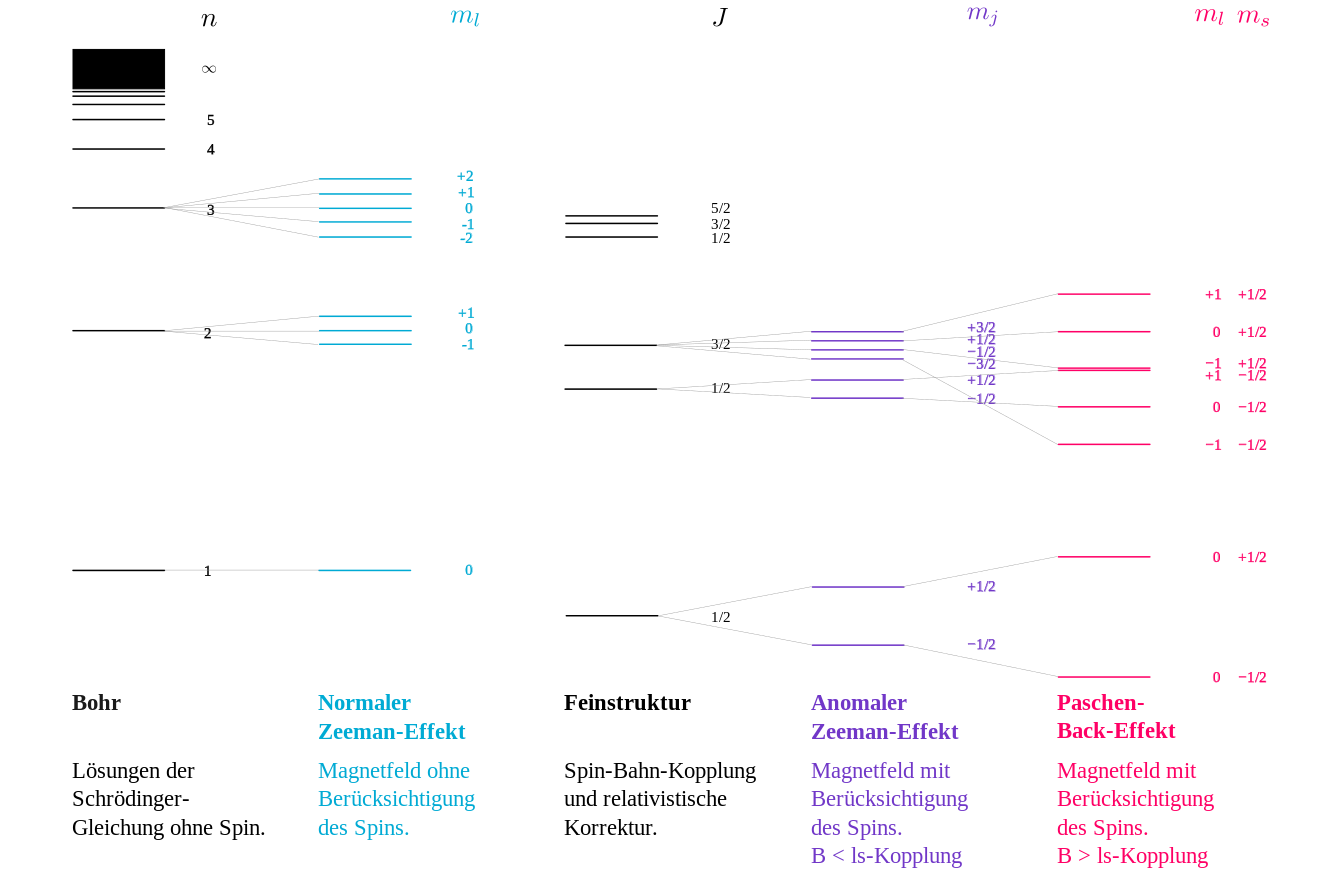
\includegraphics[width=7cm]{Bilddateien/Wasserstoff_Zeeman.svg.png}
            \caption{Aufspaltung der Spektrallinien des Wasserstoffatoms im Magnetfeld.}
        \end{figure}
        In vektorieller Darstellung ist die Entstehung von $J$ durch die Kopplung von $L$ und $S$ gegeben. Ebenso koppeln die magnetischen Momente $\mu_L$ und $\mu_S$ zu $\mu_J$, dessen Richtung jedoch im Allgemeinen nicht mehr mit derjenigen von $J$ zusammenfällt (siehe Abbildung \ref{fig:VektormodellAnomalZeeman}). Projeziert man die Vektoren $J$ und $\mu_J$ jedoch auf eine Ebene, so lässt sich mittels Trigonometrie die Projektion von $\mu_J$ auf $J$ bzw schließlich auf das Magnetfeld $B$ durch den Landé-Faktor $g$ bestimmen (siehe Abbildung \ref{fig:ProjektionVektormodellAnomalerZeeman})
        \begin{figure}[H]
            \centering
            \begin{subfigure}[b]{0.4\textwidth}
                \centering
                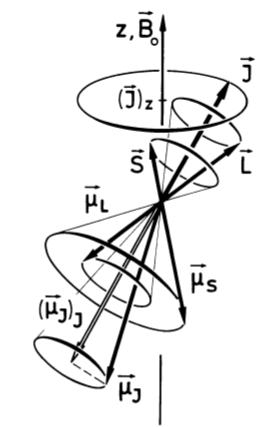
\includegraphics[height=5cm]{Bilddateien/VektormodellAnomalZeeman.png}
                \caption{Vektormodell.}
                \label{fig:VektormodellAnomalZeeman}
            \end{subfigure}
            \
            \begin{subfigure}[b]{0.4\textwidth}
                \centering
                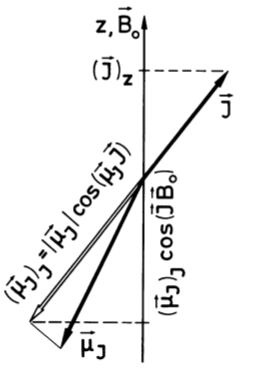
\includegraphics[height=5cm]{Bilddateien/ProjektionVektormodellAnomalerZeeman.png}
                \caption{Projektion.}
                \label{fig:ProjektionVektormodellAnomalerZeeman}
            \end{subfigure}
            \caption{Vektormodell und Projektion des anomalen Zeeman Effektes.}
        \end{figure}
        \begin{Aufgabe}
            \nr{} Schreibe eine schöne Geschichte zu diesem Thema. [$\to$ Haken-Wolf]

            \nr{} Berechne die zeitliche Mittelung von $\mu_j$. 
        \end{Aufgabe}

\end{document}